% ---------------------------------------------------------------------------
% Chapter based on a PUBLISHED paper.
% \basedon goes directly BEFORE \chapter: it prints the citation on the opener.
% \chapterauthors is kept for the A4 version but hidden in the book layout.
% \chapterabstract puts the abstract on its own page, facing a grey page.
% ---------------------------------------------------------------------------
\basedon[This chapter is based on:]{%
Lastname F.$^{*}$, Coauthor A.$^{*}$, and Coauthor B. (2025). Title of the published paper. \textit{Journal Name}, 1, 100. \url{https://doi.org/10.0000/example}}
\chapter{Full Title of the First Research Chapter, as Published}
\renewcommand{\thefigure}{\thechapter.\arabic{figure}}
\setcounter{figure}{0}

\chapterauthors{%
	Firstname Lastname$^{*}$, Author Two$^{*}$, Author Three$^{\dagger}$

	\vspace{0.5em}

	Department, University, City, Country

	\vspace{0.5em}

	\small
	$^{*}$Shared first authors.\\
	$^{\dagger}$Corresponding author: Author Three (\texttt{email@example.org})
}

\begin{chapterabstract}
[Abstract of the paper, as published.]
\end{chapterabstract}

\section{Introduction}
[Text \citep{placeholderArticle2024}.]

\section{Methods}
\subsection{Participants}
[Text.]

\paragraph{A paragraph heading.}
[Paragraph headings sit on their own line in italics.]

\subsection{Analysis}
[Text. Table~\ref{tab:ch2-example} shows a booktabs table.]

\begin{table}[htbp]
	\centering
	\caption{\textbf{Table title.} Caption text.}
	\label{tab:ch2-example}
	\begin{tabular}{@{}lcc@{}}
		\toprule
		\textbf{Measure} & \textbf{Group A} & \textbf{Group B} \\
		\midrule
		Measure 1 & 0.00 & 0.00 \\
		Measure 2 & 0.00 & 0.00 \\
		\bottomrule
	\end{tabular}
\end{table}

\section{Results}
[Text referring to Figure~\ref{fig:ch2-placeholder}.]

\begin{figure}[htbp]
	\centering
	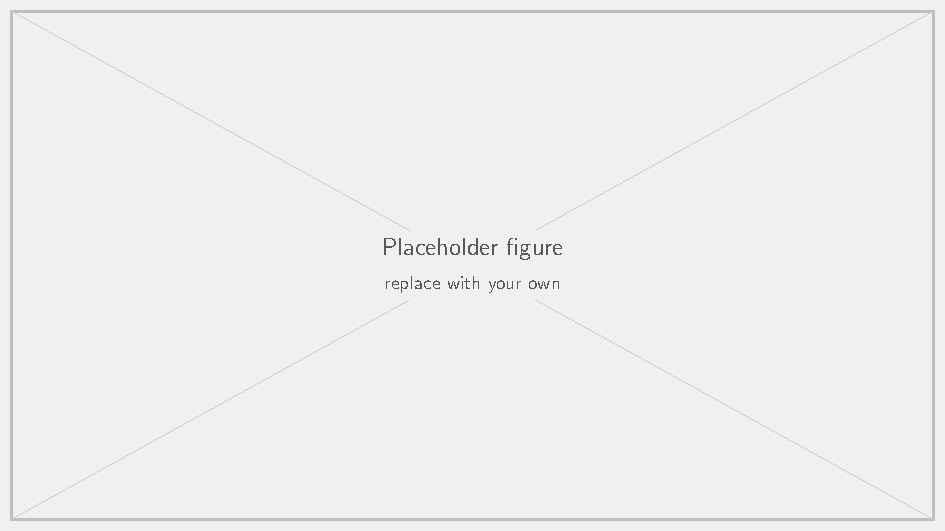
\includegraphics[width=0.9\linewidth]{chapters/chapter1/figures/placeholder.pdf}
	\caption{\textbf{Figure title.} Caption text. Keep each chapter's figures in its own \texttt{figures/} folder.}
	\label{fig:ch2-placeholder}
\end{figure}

\section{Discussion}
[Text.]

\section{Conclusion}
[Text.]

\section{Acknowledgements}
[Funding statement.]
